%===================================================================================
% JORNADA CIENTÍFICA ESTUDIANTIL - MATCOM, UH
%===================================================================================
% Esta plantilla ha sido diseñada para ser usada en los artículos de la
% Jornada Científica Estudiantil, MatCom.
%
% Por favor, siga las instrucciones de esta plantilla y rellene en las secciones
% correspondientes.
%
% NOTA: Necesitará el archivo 'jcematcom.sty' en la misma carpeta donde esté este
%       archivo para poder utilizar esta plantila.
%===================================================================================



%===================================================================================
% PREÁMBULO
%-----------------------------------------------------------------------------------
\documentclass[a4paper,10pt,twocolumn]{article}

%===================================================================================
% Paquetes
%-----------------------------------------------------------------------------------
\usepackage{amsmath}
\usepackage{amsfonts}
\usepackage{amssymb}
\usepackage{informe}
\usepackage[utf8]{inputenc}
\usepackage{listings}
\usepackage[pdftex]{hyperref}
\usepackage{graphicx}
%-----------------------------------------------------------------------------------
% Configuración
%-----------------------------------------------------------------------------------
\hypersetup{colorlinks,%
	    citecolor=black,%
	    filecolor=black,%
	    linkcolor=black,%
	    urlcolor=blue}

%===================================================================================



%===================================================================================
% Presentacion
%-----------------------------------------------------------------------------------
% Título
%-----------------------------------------------------------------------------------
\title{Informe del Proyecto Sistema de Inferencia Difusa. Simulación. Curso 2020-2021}

%-----------------------------------------------------------------------------------
% Autores
%-----------------------------------------------------------------------------------
\author{\\
\name Leonel Alejandro Garc\'ia L\'opez\email \href{mailto:r.marti@estudiantes.matcom.uh.cu}{l.garcia3@estudiantes.matcom.uh.cu}
	\\ \addr Grupo C412
}

%-----------------------------------------------------------------------------------
% Tutores
%-----------------------------------------------------------------------------------
\tutors{\\
Dr. Yudivián Almeida Cruz, \emph{Facultad de Matemática y Computación, Universidad de La Habana} \\
Lic. Gabriela Rodriguez Santa Cruz Pacheco, \emph{Facultad de Matemática y Computación, Universidad de La Habana} \\
Lic. Daniel Alejandro Valdés Pérez, \emph{Facultad de Matemática y Computación, Universidad de La Habana}}
%-----------------------------------------------------------------------------------
% Headings
%-----------------------------------------------------------------------------------
\jcematcomheading{\the\year}{1-\pageref{end}}{Leonel Alejandro Garc\'ia L\'opez}

%-----------------------------------------------------------------------------------
\ShortHeadings{Informe de Proyecto}{Leonel Alejandro Garc\'ia L\'opez}
%===================================================================================



%===================================================================================
% DOCUMENTO
%-----------------------------------------------------------------------------------
\begin{document}

%-----------------------------------------------------------------------------------
% NO BORRAR ESTA LINEA!
%-----------------------------------------------------------------------------------
\twocolumn[
%-----------------------------------------------------------------------------------

\maketitle

%===================================================================================
% Resumen y Abstract
%-----------------------------------------------------------------------------------
\selectlanguage{spanish} % Para producir el documento en Español

%-----------------------------------------------------------------------------------
% Resumen en Español
%-----------------------------------------------------------------------------------

%-----------------------------------------------------------------------------------
% English Abstract
%-----------------------------------------------------------------------------------
\vspace{0.5cm}

%-----------------------------------------------------------------------------------
% Palabras clave
%-----------------------------------------------------------------------------------

%-----------------------------------------------------------------------------------
% Temas
%-----------------------------------------------------------------------------------
\begin{topics}
	Simulación, L\'ogica Difusa
\end{topics}


%-----------------------------------------------------------------------------------
% NO BORRAR ESTAS LINEAS!
%-----------------------------------------------------------------------------------
\vspace{0.8cm}
]
%-----------------------------------------------------------------------------------


%===================================================================================

%===================================================================================
% Introducción
%-----------------------------------------------------------------------------------
\section{Introducción}
%-----------------------------------------------------------------------------------
  Como proyecto se propuso la implementaci\'on de un Sistema de Inferencia Difusa, donde deb\'iamos implementar como funciones de pertenencia la triangular o trapezoidal, dos de los m\'etodos de agregaci\'on existentes y todas las funciones de desdifusificaci\'on. Todo esto con el objetivo de implementar una librer\'ia que permita resolver un problema que a su vez valide librer\'ia o sistema propuesto.

%===================================================================================

\subsection{Estructura}

 El proyecto est\'a estructurado por las carpetas \textbf{doc} y \textbf{fuzzy\_logic\_sytem}, para la documentaci\'on y la implementaci\'on del sistema respectivamente, en la ra\'iz del proyecto se encuentra contenido tambi\'en en un archivo py \textbf{main.py} el problema que me propuse a resolver, para demostrar la utilizaci\'on de mi librer\'ia.
 
\subsection{Implementaci\'on}
Ahora introduci\'endonos en la implementaci\'on, sobre el \textbf{fuzzy\_logic\_sytem} a continuaci\'on una disertaci\'on de cada una de sus partes. 

\subsection*{Conjuntos Difusos}

 Como primera entidad crucial en este sistema definimos conjunto Difuso en la clase abstracta \textit{FuzzySet} que solo contiene un nombre, y una funci\'on de membres\'ia, luego una implementaci\'on concreta de este conjunto difuso te\'orico, el \textit{CustomizableFuzzySet} que permite adem\'as especificar un dominio de definici\'on, una funci\'on de membres\'ia y una lista de puntos definitorios para la funci\'on y el conjunto dominio, se le defini\'o el operador de \textit{+} para realizar de una forma legible la uni\'on entre conjuntos, que da como resultado otro definido en la clase \textit{UnionFuzzySet} que hereda de la anterior definici\'on y que no es m\'as que la uni\'on de los dominios, y las funciones de membres\'ia aplicadas con una \textit{t-conorma} pasada como argumento (por defecto tiene \textit{t-conorma}=\textit{max()}).
 
 
 Otras implementaciones particulares de esta clase \textit{CustomizableFuzzySet}, fueron una para cada funci\'on de membres\'ia siguiente:
 

 \begin{itemize}
 	\item \textit{GammaFuzzySet}, 
 	\item \textit{LFuzzySet} (funci\'on \textit{l} opuesta de \textit{gamma}), 
 	\item \textit{LambdaFuzzySet} (tambi\'en llamado \textit{TriangleFuzzySet}), 
 	\item \textit{TrapezoidalFuzzySet} (tamb\'en llamado \textit{PiFuzzySet}), 
 	\item \textit{SigmoidalFuzzySet} (\textit{sigmoidal} o funci\'on \textit{s}), 
 	\item \textit{ZFuzzySet} (funci\'on \textit{z} opuesta de \textit{s})
 	\item \textit{GaussianFuzzySet} (definida como una composici\'on de las funciones \textit{z} y \textit{s})
 \end{itemize}

\subsection*{Variable Lingüística}
 La siguiente definici\'on implementada fue la de variable lingüística, encapsulada en la clase \textit{LanguageVariable} que posee un nombre, y un conjunto de conjuntos difusos que caracterizan la propiedad o rasgo representada por la variable. Esta almacena y permite el acceso a los grados de pertenencia (para los conjuntos que contiene) de forma sencilla, por medio de su m\'etodo \textit{fuzzify}. Es importante aclarar que defin\'i el operador m\'odulo (\textit{\%}) para una sintaxis mas fluida al expresar una operaci\'on que como resultado retorna un valor num\'erico entre 0 y 1 como valor o grado de pertenencia.

 \subsection*{Preposiciones o Antecedentes}
 Para la construcci\'on de proposiciones nos definimos una jerarqu\'ia de \textit{FuzzyProposition} siendo esta la clase abstracta ra\'iz, que contiene implementaciones de las sobrecargas para los operadores \textit{|} (operaci\'on \textit{or} entre preposiciones), el \textit{\&} (operaci\'on \textit{and}) y el operador \textit{~} o \textit{invert} (operaci\'on \textit{not} que resulta en el valor opuesto de la funci\'on de pertenencia $~f(x)=1-f(x)$).Esta clase tambi\'en permite especificar una \textit{tnorma} y \textit{tconorma} que por defecto esta definida con \textit{min} y \textit{max} respectivamente.

 De esta clase se derivan implementaciones para las operaciones binarias, (\textit{AndFuzzyProposition} y \textit{OrFuzzyProposition}), como para las unarias (\textit{MembershipProposition}, y \textit{NotFuzzyProposition})
 
 \subsection*{Reglas}
 Luego, viene una composici\'on, regla difusa \textit{FuzzyRule}, la cual esta conformada por un \textit{proposition} o antecedente, un \textit{consecuente} y un \textit{method\_transformer} o m\'etodo de transformaci\'on aplicable a conjuntos difusos que puede estar especificado o no, este es utilizado para obtener los conjuntos difusos transformados para el procesamiento de \textit{Larsen} o \textit{Mamdani} en cada uno de las variables resultantes (del consecuente) de cada regla. Esta definici\'on tambi\'en est\'a compuesta por un m\'etodo \textit{evaluate} que por defecto retorna el valor resultante de evaluar la preposici\'on y un diccionario de \{\textit{nombre\_de\_variable\_lingüística}:
 \textit{conjunto\_difuso\_transformado}\}, y puede ser sobrescrito para utilizar otros m\'etodos de inferencia.
 
 A partir de este \textit{FuzzyRule}, derivan dos implementaciones una regla  \textit{LarsenRule} para solucionar por el m\'etodo de agregaci\'on de \textit{Larsen} y otro \textit{MamdaniRule} para la resoluci\'on por \textit{Mamdani}. Notar que para facilitar las operaciones de escalado y corte que realizan estos m\'etodos sobre los conjuntos de consecuentes en cada regla result\'o sencillo apoyarnos en la extensible clase \textit{CustomizableFuzzySet}, implementando as\'i \textit{MamdaniCut} y \textit{LarsenScale}.
  
 Llegados a este punto tenemos reglas que lucen de esta forma:

\begin{figure}[h]	
	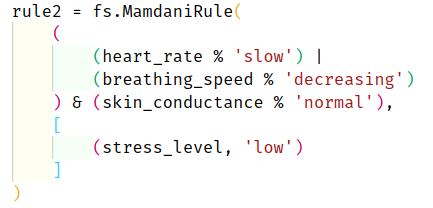
\includegraphics[scale=.7]{mamdani-rule.png}
\end{figure}
\subsection*{Sistema de inferencia}
	Por \'ultimo est\'a la clase que enlaza todas las partes, donde la inferencia se realiza, \textit{FuzzyInferenceSystem}
	que recibe en su constructor un listado de todas las reglas definidas. Para a partir de su m\'etodo \textit{infer} que recibe un diccionario de valores de entrada para evaluar las reglas, una \textit{t-conorma} que por defecto es \textit{max} y un m\'etodo de desdifusificaci\'on que por defecto es \textit{centroide\_dediffusion}, obtener un diccionario con el valor final de todas las variables de los consecuentes.

 \subsection*{Desdifusificaci\'on}
 
 Para obtener una respuesta por los m\'etodos de agregaci\'on \textit{Mamdani} y \textit{Larsen} es necesario aplicar uno de los m\'etodos desdifusificaci\'on entre los implementados, el utilizado en proyecto como por defecto es el m\'etodo del \textit{Centroide} a continuaci\'on un listado de los implementados:
 
 \begin{itemize}
 	\item \textbf{Smallest of Maximum}: genera el menor $x$ donde se alcanza el m\'aximo.
 	\item \textbf{Largest of Maximum}: genera el mayor $x$ donde se alcanza el m\'aximo.
 	\item \textbf{Middle of Maximum}: genera el promedio de aquellos valores de control $x$ donde se alcanza el m\'aximo.
 	\item \textbf{Centroide}: genera el centro de gravedad de los conjuntos que conforman la agregaci\'on.
 	\item \textbf{Bisection}: genera el valor $x$ tal que particiona el \'area en dos regiones iguales.
 
 \end{itemize}
%===================================================================================
% Desarrollo
%-----------------------------------------------------------------------------------
\section{Consideraciones}
La forma en que se estructur\'o e implement\'o este sistema fue con la idea de hacerlo sostenible en el tiempo, fuera f\'acil de usar y tuviera una sintaxis simple de leer. Como idea inicial se pens\'o en separar la definici\'on de un conjunto difuso de su funci\'on de membres\'ia, pero como el concepto de ambos est\'a muy entrelazado encontr\'e pertinente su unificaci\'on en una sola clase, que a su vez encapsula toda la funcionalidad de un conjunto difuso, y lo hace f\'acilmente extensible y modificable.
  
%-----------------------------------------------------------------------------------
 \section{Problema Planteado}
 \subsection{Detector de Mentiras}	
  Para este problema se presuponen condiciones \'optimas del ambiente donde se realizan las mediciones, as\'i como tambi\'en que los sujetos no padezcan hipertensi\'on o hipotensi\'on arterial, hiperhidr\'osis u otra afecci\'on que altere los rangos promedio que en este ejemplo se prefijan (de otra forma deben ser modificados los rangos de las variables). Los sujetos sospechosos al ser interrogados es dif\'icil determinar cuando est\'an o no mintiendo. Dado este tipo de situaciones se les conectan por medio de sensores al cuerpo, a una m\'aquina (pol\'igrafo) le hacen una pregunta al interrogado y a partir de los resultados obtenidos en ese intervalo de tiempo y una grado de \textit{credibilidad} aportado por el interrogador, conforman un \textit{veredicto} sobre la veracidad de las palabras del cuestionado.
  
  Las variables lingüísticas que en este proceso intervienen, con las respectivos conjuntos que representan, las muestro a continuaci\'on:
  \begin{itemize}
  	\item \textit{Credibilidad} (grado): 
  		\subitem  \textit{credible}:  \textit{Sigmoidal}, domain$(0,10)$
  	\item \textit{Frecuencia Card\'iaca} (beats/min):  
  		\subitem \textit{slow}: \textit{l}, domain$(0,70)$
  		\subitem \textit{medium}: \textit{trapezoidal}, domain$(55,120)$
  		\subitem \textit{fast}: \textit{gamma}, domain$(110,180)$
   	\item \textit{Presi\'on Sangu\'inea Sist\'olica} (mmHG): 
   		\subitem \textit{normal}: \textit{z}, domain$(70,120)$
   		\subitem \textit{slightly-high}: \textit{gaussiana}, domain$(110,140)$
   		\subitem \textit{high}: \textit{sigmoidal}, domain$(130,180)$
  	\item \textit{Presi\'on Sangu\'inea Diast\'olica} (mmHG): 
  	    \subitem \textit{normal}: \textit{z}, domain$(50,90)$
		\subitem \textit{slightly-high}: \textit{gaussiana}, domain$(75,95)$
		\subitem \textit{high}: \textit{sigmoidal}, domain$(90,110)$
  	\item \textit{Velocidad Respiratoria} (grado de cambio):  
  		\subitem \textit{decreasing}: \textit{z}, domain$(-10,0)$
  		\subitem \textit{constant}: \textit{gaussiana}, domain$(-2,2)$
  		\subitem \textit{increasing}: \textit{sigmoidal}, domain$(0,10)$
  	\item \textit{Conductancia de la piel}(grado): 
  		\subitem \textit{normal}: \textit{z}, domain$(0,10)$
  		\subitem \textit{high}:	\textit{sigmoidal}, domain$(8,20)$
  \end{itemize}
  Variables lingüísticas resultantes:
  \begin{itemize}
		\item \textit{Nivel de estr\'es} (grado):
			\subitem \textit{low}:	\textit{z}, domain$(0,45)$
			\subitem \textit{medium}:	\textit{gaussiana}, domain$(3,7)$
			\subitem \textit{high}:	\textit{sigmoidal}, domain$(5.5, 10)$
		\item \textit{Veredicto} (grado):
			\subitem \textit{lying} \textit{z}, domain$(0, 5.5)$
			\subitem \textit{not\_lying} \textit{sigmoidal}, domain$(4.5, 10)$
  \end{itemize}
  
  Ahora las reglas definidas para este problema pueden ser tan complejas como uno desee, pero por simplificar las explicaci\'on a continuaci\'on un sumario de la sem\'antica detr\'as de cada regla:
  \begin{itemize}
  	\item[Rule1] Si alguno de los par\'ametros utilizados para medir la respuesta corporal tiene valores altos, entonces considero que potencialmente se trata de una mentira y el estr\'es provocado es alto.
  	\item[Rule2] Si alguno de los par\'ametros utilizados para medir la respuesta corporal tiene valores muy bajos, considero que potencialmente se trata de bajo estr\'es provocado y nada que decir de la veracidad.
  	\item[Rule3] Si los par\'ametros utilizados para medir la presi\'on arterial arrojan resultados estables, considero que el nivel de estr\'es es bajo y no esta mintiendo.
  	\item[Rule4] Si los par\'ametros utilizados para medir la presi\'on arterial arrojan resultados ligeramente altos, considero que el estr\'es esta en un nivel medio y nada que aportar a la veracidad.
  	\item[Rule5] Si los par\'ametros utilizados para medir la presi\'on arterial arrojan resultados altos, considero que el estr\'es esta en un nivel alto tambi\'en y es una potencial mentira
  	\item[Rule6] Esta secci\'on va centrada en si alguno de los 3 valores de Ritmo Card\'iaco, Velocidad Respiratoria o Conductancia de la piel es alto, y tiene otro de estos que se encuentra en la medida de lo normal (medianamente alto), todos implican a que el nivel de estr\'es es medio y se trata de una mentira:
  	
  		\subitem Rule6.1 Si la Conductancia de la piel es alta (sujeto sudoroso), con un Ritmo Card\'iaco estable o una Respiraci\'on constante.
  		\subitem Rule6.2 Si el Ritmo Card\'iaco es r\'apido, con una Conductancia de la piel normal o una Respiraci\'on constante.
  		\subitem Rule6.3 Si la Velocidad Respiratoria aumenta, con una Conductancia de la piel normal o un Ritmo Card\'iaco estable.
  	\item[Rule7] Si los par\'ametros utilizados para medir el Ritmo Card\'iaco y la Velocidad Respiratoria arrojan resultados de un comportamiento estable, considero entonces que estamos en un caso de estr\'es medio y el sujeto no esta mintiendo.
  	\item[Rule8] Si los par\'ametros utilizados para medir el Ritmo Card\'iaco y la Velocidad Respiratoria arrojan resultados de un comportamiento medianamente bajos, con una Conductancia normal, considero entonces que estamos en un caso de estr\'es bajo y el sujeto no esta mintiendo.
  	\item[Rule9] Si la respuesta recibida aporta Credibilidad, considero que es veraz la misma, no se esta mintiendo.
  	\item[Rule10] Si la respuesta recibida carece de sentido, considero que estamos en presencia de una mentira.
  \end{itemize}
  
  
\subsection{Resultados Obtenidos}
	En ambiente ideal, los resultados arrojados por \textit{Mamdani} respecto a las reglas anteriormente descritas, los resultados fueron los esperados, a continuaci\'on algunos ejemplos.
	
	Para un estado corporal estable, comportamiento calmado y una credibilidad discreta, se obtiene un grado de vericidad en el rango de lo ver\'idico pero con resultados no tan impresionantes:
	\begin{verbatim}
		--------------------------------------------------
		VALUES:
		Degree of Credibility (appreciation) [0, 10]:       6
		Heart Rate (BEATS/MINUTES) [30, 180]:              50
		Blood Systolic Pressure (mmHg) [90, 180]:         100
		Blood Diastolic Pressure (mmHg) [60, 110]:         70
		Breathing Speed (Degree) [-10, 10]:                 2
		Skin Conductance (relating with the sweat) [0, 20]: 5
		--------------------------------------------------
		CONCLUSIONS:
		StressLevel: 2.00 / 10
		Veredict:    5.91 / 10
	\end{verbatim}
	Para un estado corporal inestable y nervioso, con una credibilidad por debajo de la media pero no tan pronunciada, tenemos los siguientes:
	
	\begin{verbatim}
		--------------------------------------------------
		VALUES:
		Degree of Credibility (appreciation) [0, 10]:        4
		Heart Rate (BEATS/MINUTES) [30, 180]:               75
		Blood Systolic Pressure (mmHg) [90, 180]:          110
		Blood Diastolic Pressure (mmHg) [60, 110]:          90
		Breathing Speed (Degree) [-10, 10]:                  4
		Skin Conductance (relating with the sweat) [0, 20]: 10
		--------------------------------------------------
		CONCLUSIONS:
		StressLevel: 5.65 / 10
		Veredict:    3.85 / 10
	\end{verbatim}
	
 \section{Conclusiones}
 Ya en este punto se hace evidente la utilidad de la l\'ogica difusa en variedad de problemas, sobre todo en la interpretaci\'on no binaria de la realidad, que reduce la complejidad para tomar decisiones y desarrollar sistemas complejos que se destacan en la automatizaci\'on de procedimientos reactivos con sistemas de medida gradual.
\end{document}

%===================================================================================
